\section{Password Authentication}

Passwords are one of the most common and oldest forms of end user authentication, being first used in computers at MIT in the mid-60s \cite{mcmillan2012password}.

We need to understand the high level model of authentication model of password authentication, and solutions to overcome their weaknesses.

\subsection{Authentication Model}

% High level arch
Password based authentication is a simple authentication model, based on a shared secret between a user and a system. 
The secret (password) is often used in a combination with a user ID. 
The password itself is usually a set of characters or words memorised by the user, and inputted via a keyboard.

To authenticate, the user exchanges the password with the system via a keyboard interface, and the system authenticates the user according to passwords validity.

\begin{figure}[h]
	\centering
	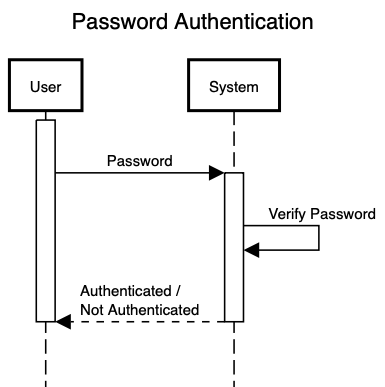
\includegraphics[height=6cm]{images/password-authentication}
	\caption{Password Authentication Model}
	\label{fig:password-authentication}
\end{figure}


% Security considerations
\subsection{Security}

Security of any authentication system is defined by is security against many attack vectors, these can be split into two groups in relation to our authentication method.
General attack vectors exist in any authentication system, regardless of the specific authentication mechanism, these include (but not limited to) insecure network communication, compromised host systems, phishing, etc. For example, an authentication system would be insecure if an attacker could eavesdrop to the communication between the user and the system, or a malicious program on the clients system could intercept the password before being sent, a user could compromised his password by mistakingly sending it to a phishing website.

We are going to assume participating systems and network are secure agains general threats and are going to focus on attack vectors specific to a common password authentication system implementation.

In a common password authentication system implementation used on the web the user sends a plain-text password over a secure HTTPS connection, the server verifies it according to an internal mechanism and responds.


\subsubsection{Vulnerabilities}

The simplicity that makes passwords practical for users is what makes them especially vulnerable for systems that use them.

Because passwords are supposed to be memorised and the proliferation of different websites requiring them, users tend to pick password that are easier to remember and reuse passwords across different websites \cite{conklin2004password}.
Many websites also don't properly handle and store passwords or are insecure in some other ways, enabling attackers to steal users plain-text passwords when a security breach happens.

Attacks can be according to NIST \cite{grassi2017} classified as \textit{online} or \textit{offline}, based on wether the attacker is directly interacting with an authentication system.

\paragraph{Online Attacks} A form of an \textit{active attack}, where an attacker is attempting bypass authentication by directly interacting with the system.
These attacks are usually very \textit{noisy}, making it easy for an authentication system to detect an attack is happening, and prevent it.
This makes online attacks much less effective than offline ones.

For example, with a simple brute-force method an attacker can try random passwords to authenticate into a single user account.
An authentication system can detect an attack is happening because of the high number of failed authentication attempts, or some other security triggers. If the system knows it's under attack it can react to it making it ineffective.

Real life methods of online attacks rely on operating under the radar of detection, for example, by trying out a small number of passwords on each user.
Such popular methods are \textit{password spraying} and \textit{credential stuffing}, both of which utilise information from data breaches, like lists of most commonly used passwords, or username and password combinations.
\textit{Password spraying} is taking a small number of commonly used passwords and attempting to authenticate with a large number of accounts, the attacker is assuming that in a large sample of accounts some will be using common passwords.
\textit{Credential stuffing} is taking a leaked user credential, for example a username and password combination found in a data breach, and using them to authenticate into multiple websites. 
The attacker is assuming that if a person is using a set of credentials on one website, they are potentially reusing them on other websites.

\paragraph{Offline Attacks} 
A form of a passive attack performed in a system controlled by the attacker.
For example, an attacker might analyse data on his personal computer to extract sensitive information. The data is obtained by either theft of file, eavesdropping an authentication protocol or a system penetration.

\textit{Password cracking} is method of extracting user credentials from data used by the authentication system to verify users credentials.
The success of password cracking is generally determined by two factors, that influence the time required to guess the password.

\subparagraph{Password Handling}
Password handling describes how passwords are stored at rest and used in the verification process.

A naive system might store the passwords or password-equivalent data in plain text and compare them for verification, while simple this system is insecure as user credentials directly are exposed with any unauthorised access.

A common approach today is to use methods of \textit{password hashing} to derive a password digest that is then stored in the database. 
When verifying the password is hashes again, and the digests are compared.

Using pure hashing functions like SHA family is discouraged because they designed to run fast and can be accelerated with ASIC chips, making them vulnerable to pre-computed hash tables.
A better solution are password key-derivation functions. 
Algorithms utilising hash functions designed with the purpose of being both time-consuming and memory-hard, examples of such tools are Argon2 \cite{biryukov2016argon2}, Scrypt \cite{percival2016scrypt} and Balloon \cite{boneh2016balloon}.
Using an extra value called \textit{salt} \cite{hornby2016salted} prevents attacks with pre-computed hash tables.
Because salt is stored alongside password hashes, systems sometimes also utilise a third value called \textit pepper, which is the same for all passwords, but stored in a different place from the salt.


\subparagraph{Password Strength}
Measure of information entropy and the difficulty of the password being guesses or brute-forced.
Re-using passwords greatly undermines password strength and is what attacks like credential stuffing rely on.
Have I Been Pwned \cite{hunt2021have} catalogs 613,584,248 passwords recovered from data breaches, while CrackStation \cite{hornby2019password} lists a collection of 1,493,677,782 words used for password cracking.